\chapter{Eksperymenty i wyniki}

W tym rozdziale zaprezentowano wyniki przeprowadzonych eksperymentów oraz ich analizę. Skupiono się na ocenie najlepszego modelu, wpływie parametrów treningowych  oraz funkcji nagrody na proces uczenia i końcowe wyniki agenta.

\section{Wyniki najlepszego modelu}

Najlepszy model został wybrany na podstawie maksymalnej średniej nagrody.

\begin{figure}[!ht]
	\centering
	
\includegraphics[width=\textwidth]{plots/pos.eps}
	\caption{Wyniki najlepszego modelu: pozycja agenta naniesiona na mapę poziomu\(x_{\text{pos}}\).}
	\label{fig:best_model_results}
\end{figure}

Model osiągnął maksymalną pozycję \(x_{\text{pos}}\) wynoszącą \(1151\) (około \(\frac{1}{3}\) poziomu) oraz średnią nagrodę \(127.718\) na epizod po 2560 epizodach.

\section{Proces trenowania}

Podczas trenowania modelu agent stopniowo uczył się strategii pozwalających na skuteczniejsze poruszanie się po poziomie w grze \textit{Super Mario Bros}. Na rysunku~\ref{fig:training_process} przedstawiono wykres ilustrujący maksymalną osiągniętą pozycję \(x_{\text{pos}}\) w funkcji liczby epizodów.

\begin{figure}[!ht]
	\centering
	\includegraphics[width=0.8\textwidth]{plots/max_x.eps}
	%\includegraphics[width=0.8\textwidth]{training_process.png}
	\caption{Proces trenowania: maksymalna pozycja \(x_{\text{pos}}\) w zależności od liczby epizodów.}
	\label{fig:training_process}
\end{figure}

\paragraph{Wnioski:}

Wzrost wartości \(x_{\text{pos}}\) w trakcie trenowania nie jest liniowy, co jest wynikiem złożoności środowiska oraz charakterystyki procesu uczenia:
\begin{itemize}
	\item \textbf{Złożoność środowiska gry:} W grze agent napotyka różnorodne przeszkody i przeciwników, które wpływają na jego zachowanie. W niektórych epizodach agent może trafić na sytuacje, których wcześniej nie doświadczył, co prowadzi do spadku wyników.
	\item \textbf{Duża przestrzeń wejściowa:} Relatywnie wysoka liczba pikseli w obrazie wejściowym (\(60 \times 64\)) powoduje, że model musi analizować znaczną ilość informacji, co utrudnia szybkie generowanie optymalnych strategii.
	\item \textbf{Eksploracja i eksploatacja:} Strategia \(\epsilon\)-greedy sprawia, że w początkowych etapach agent częściej eksploruje nowe akcje, co prowadzi do spadku wyników w epizodach, gdzie nowe strategie okazują się nieskuteczne.
	\item \textbf{Dynamiczny charakter nagród:} Model jest nagradzany za różnorodne aspekty gry (prędkość, postęp, eliminację przeciwników). Równoczesna optymalizacja wielu składników funkcji nagrody może prowadzić do okresowych spadków wyników, gdy agent próbuje dostosować swoje działania.
\end{itemize}

Pomimo tych trudności, ogólny trend wskazuje na stały wzrost wartości \(x_{\text{pos}}\) w dłuższym okresie. Spadki są naturalnym elementem procesu uczenia w złożonych środowiskach, ponieważ agent dostosowuje swoje strategie do coraz bardziej wymagających sytuacji w grze.

\section{Porównanie różnych wartości wygaszania \(\epsilon\)}

Eksperymenty przeprowadzono dla trzech różnych schematów wygaszania \(\epsilon\):
\begin{itemize}
	\item \textbf{Za szybkie wygaszanie:} Początkowe \(\epsilon = 1.0, \epsilon_d=0.95\), wygaszanie w \(76\) krokach.
	\item \textbf{Optymalne wygaszanie:} Początkowe \(\epsilon = 1.0, \epsilon_d=0.994\), wygaszanie w \(765\) krokach.
	\item \textbf{Za wolne wygaszanie:} Początkowe \(\epsilon = 1.0, \epsilon_d=0.997\), wygaszanie w \(1500\) krokach.
\end{itemize}

Na rysunku~\ref{fig:epsilon_comparison} przedstawiono wpływ różnych schematów na średnią nagrodę oraz wartość funkcji kosztu.

\begin{figure}[!ht]
	\centering
	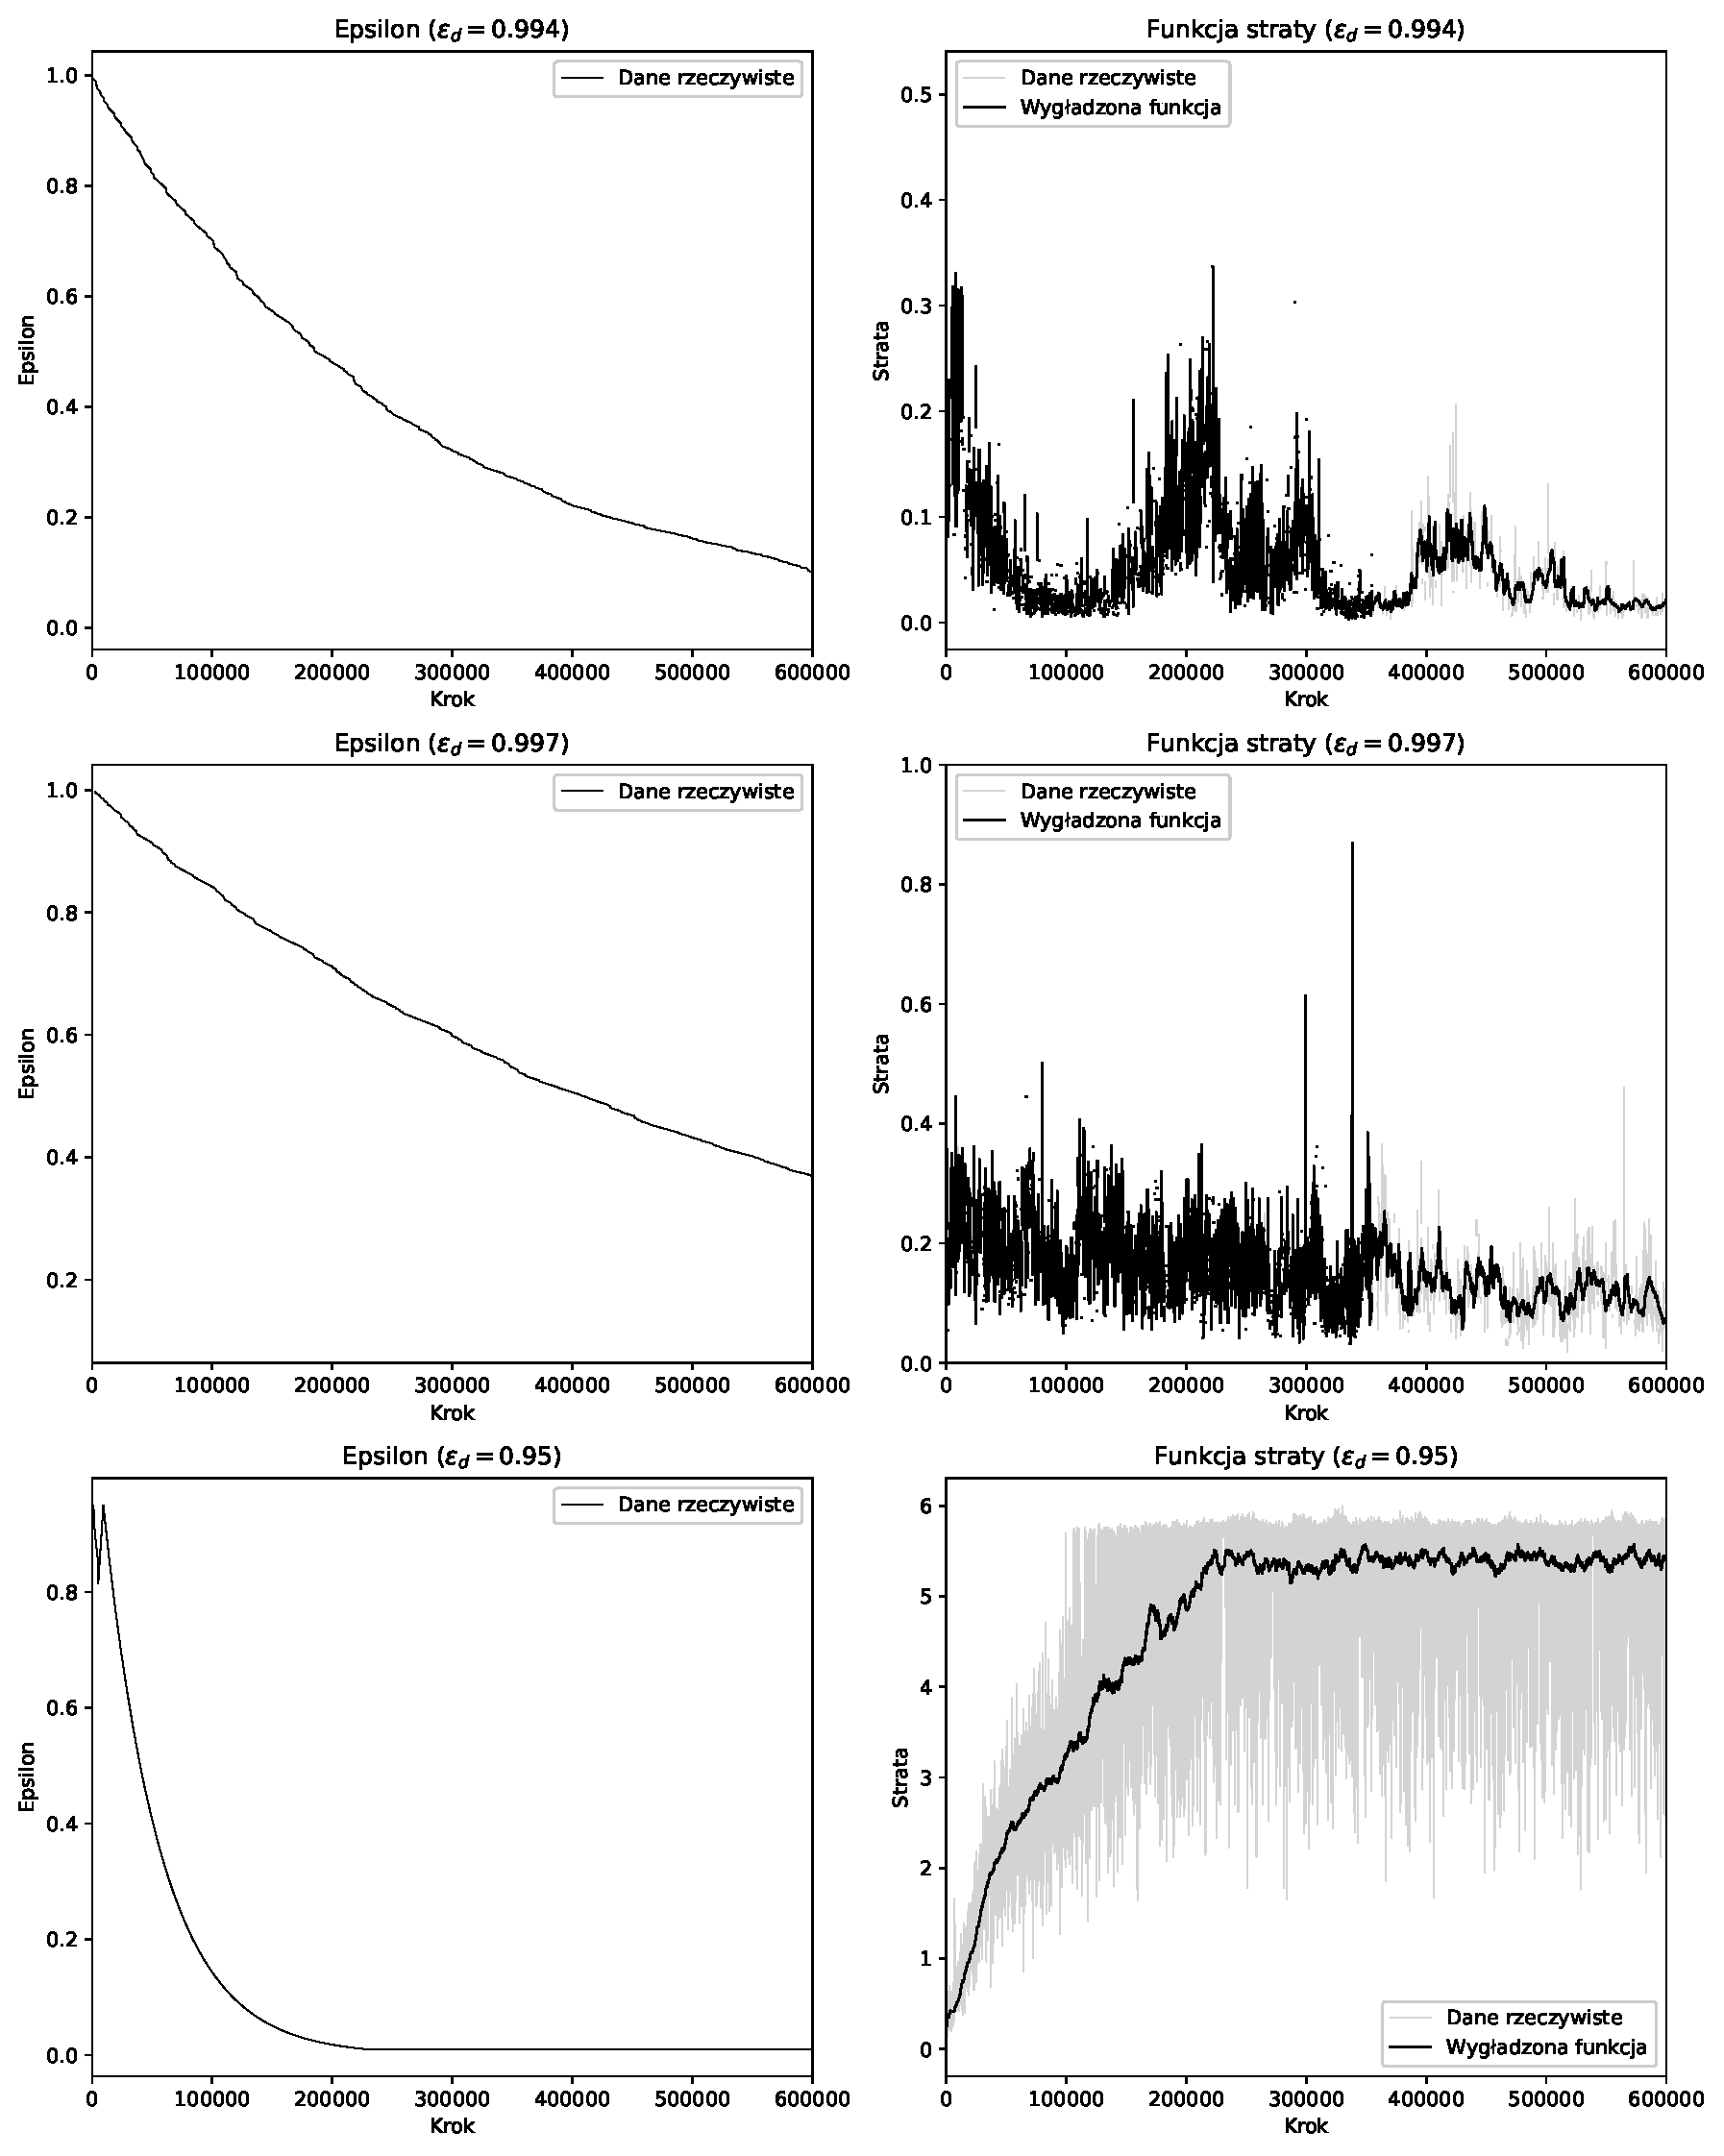
\includegraphics[width=\textwidth]{plots/epsilon.eps}
	\caption{Porównanie wpływu różnych schematów \(\epsilon\) na nagrodę (lewy wykres) i stratę (prawy wykres).}
	\label{fig:epsilon_comparison}
\end{figure}

\paragraph{Wnioski:}
Zbyt szybkie wygaszanie powodowało, że agent nie nadążał z eksploracją, co prowadziło do wysokiej wartości funkcji kosztu, która nie wracała do niższych wartości. Z kolei zbyt wolne wygaszanie znacząco wydłużyło czas uczenia. Model ze zbyt szybkim wygaszaniem \(\epsilon\) niedostatecznie zeksplorował własne środowisko i ostatecznie nie dokonał żadnych zmian co do rezultatów.

\section{Wpływ funkcji nagrody}

Eksperymenty dotyczyły modyfikacji funkcji nagrody poprzez manipulację wagami nagrody za prędkość (\texttt{speed}) i pozycję (\texttt{position\_reward}). Na rysunku~\ref{fig:reward_comparison} przedstawiono maksymalne wartości \(x_{\text{pos}}\) dla różnych konfiguracji.

\begin{figure}[!ht]
	\centering
	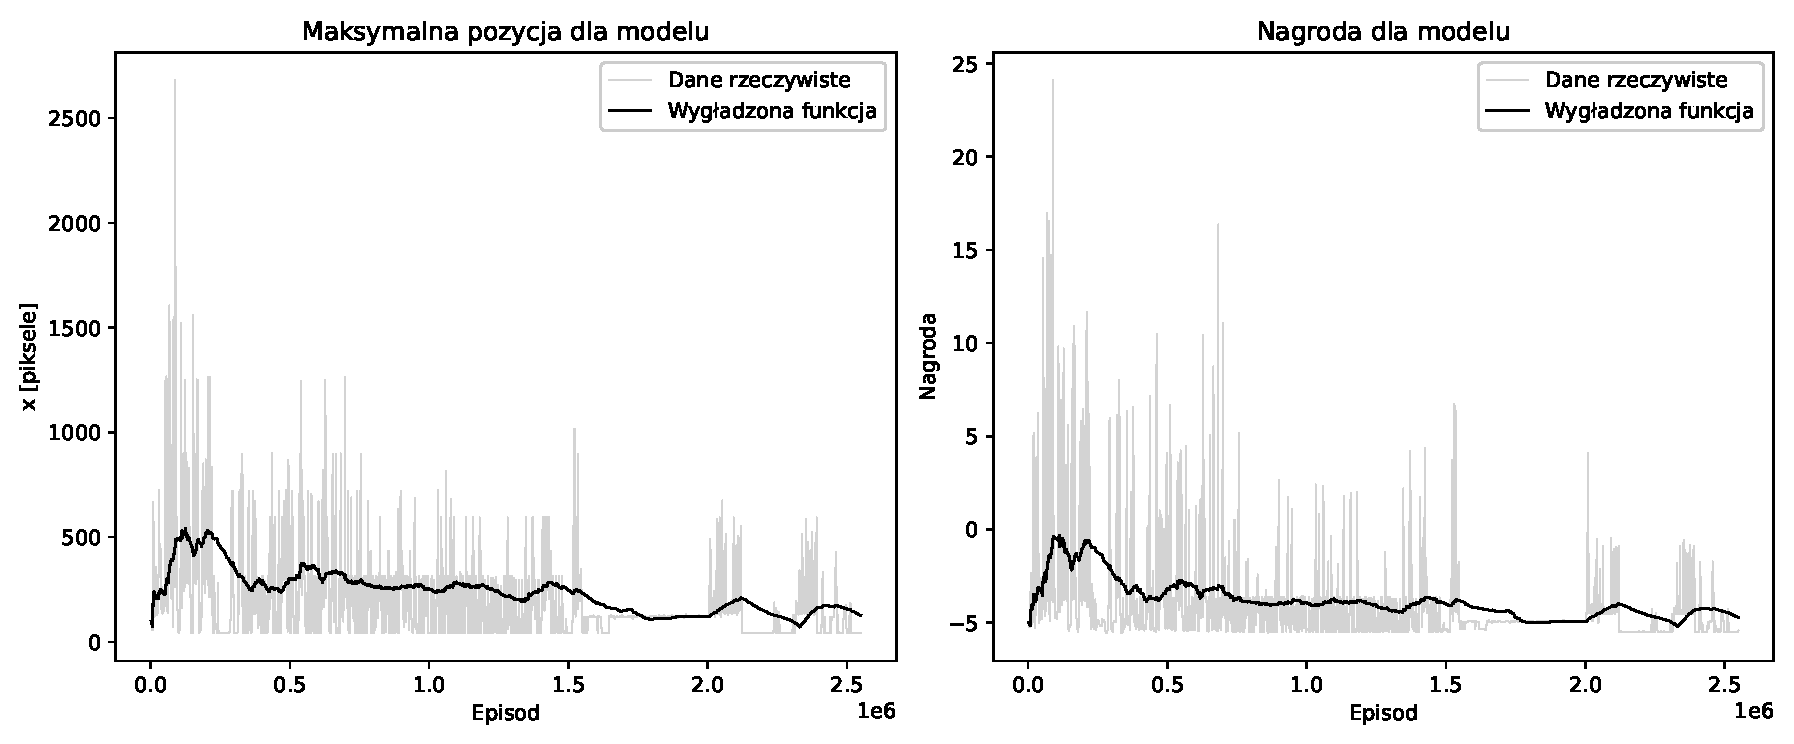
\includegraphics[width=\textwidth]{plots/reward.eps}
	%\includegraphics[width=0.8\textwidth]{reward_function_comparison.png}
	\caption{Wpływ funkcji nagrody na maksymalną pozycję \(x_{\text{pos}}\).}
	\label{fig:reward_comparison}
\end{figure}
\paragraph{Wnioski:}

Eksperymenty wykazały, że niewłaściwy dobór funkcji nagrody znacząco wpływa na skuteczność procesu uczenia. Jeśli nagroda była skoncentrowana wyłącznie na pozycji \(x_{\text{pos}}\), agent priorytetowo traktował poruszanie się w poziomie, ignorując inne aspekty gry, takie jak unikanie przeciwników czy eksploracja otoczenia. Prowadziło to do sytuacji, w której model uczył się niskiej jakości strategii, szybko osiągając maksymalne wartości nagrody, ale z pominięciem ważnych elementów gry.

Z kolei zbyt wysokie kary, takie jak te wynikające z dużych wartości ujemnych za śmierć lub przekroczenie czasu, skutkowały spadkiem stabilności procesu uczenia. Agent unikał eksploracji, obawiając się wysokich strat, co prowadziło do lokalnych minimów w funkcji wartości \(Q(s, a)\). W rezultacie model nie potrafił poprawnie uczyć się złożonych strategii, a maksymalne wartości \(x_{\text{pos}}\) osiągane w trakcie treningu były znacznie niższe.

Optymalne wyniki uzyskano, gdy funkcja nagrody była dobrze zbalansowana — uwzględniała zarówno postęp w poziomie (\(x_{\text{pos}}\)), jak i inne kluczowe aspekty, takie jak prędkość czy unikanie ryzyka. Takie podejście pozwoliło agentowi na bardziej zrównoważony rozwój strategii, co przełożyło się na wyższe wartości \(x_{\text{pos}}\) oraz stabilniejszy proces uczenia.

\section{Podsumowanie wyników}

Eksperymenty wykazały, że:
\begin{itemize}
	\item Optymalne wygaszanie \(\epsilon\) oraz \(\gamma = 0.994\) zapewniały stabilny proces uczenia.
	\item Manipulacja funkcją nagrody pozwalała na dostosowanie zachowania agenta, ale wymagała równowagi między różnymi składnikami nagrody.
\end{itemize}
